%!TEX root = thesis.tex

\chapter{Information Based Evacuation Agent Architecture: IBEVAC}
\label{chapter:IBEVAC}

In the previous chapter, the salient features of the behavior of a crowd engaging in egress during a fire evacuation were introduced. Firstly, it is understood that people don't immediately exit a building on hearing a fire alarm or seeing smoke. The occupant gets only an inkling about the danger that is possible. In both these cases there is not enough \emph{information} for him to get scared and make the decision to egress. If the cues are interesting enough, he then embarks on investigating to gather more \emph{information}. When he realizes that the situation requires some action, he tries to escape. However, he does not try to go directly to the exit. Instead, he first tries to meet up with his primary group members~(provided he has one)~\cite{Sime:1983uy,Torres:2010tj,Cornwell:2003uo,Aveni:1997wq} and only when he is with all of them do they all try to exit together. While trying to exit, \emph{information} still plays an important part. Firstly, unless he is trained for egress, it is unlikely that he will have knowledge of all the exits. As a result, he is most likely to just move to the nearest exit that he knows of. He may change his exit choice if he gains new information either through signs he perceive or through communication with other people engaging in egress~(including his own group or personnel in charge of evacuating the place). Time constraints and stress can create distortions in the capacity to process information and produce what seems to an outsider to be irrational behavior~(even though it is still rational within the decision maker's frame of knowledge). An overview of this process of human evacuation is illustrated in Fig.~\ref{fig:EvacuationProcess}. Whatever action they are undertaking, they preserve social norms as far as possible by not shoving or pushing other people~\cite{Cocking:2005uc,Drury:2009ga,Torres:2010tj}.
\begin{figure}[!htb]
\centering
\includegraphics[height=4in]{fig-ProcessOfEvacuation}
\caption[The Process of Evacuation]{The Process of Evacuation: This state diagram shows the different phases of behavior of a person engaging in egress and the triggers that cause phase changes}
\label{fig:EvacuationProcess}
\end{figure}

It is generally recognized that information plays an important part in solving problems~\cite{Simon:1970th} and other daily decisions. Chapter~\ref{chapter:IBP} explains how information has an important role to play not only in high level decision making but also at the lower level of perception and simple motion. The behavioral model proposed in this report is based on the idea that humans are \emph{``serial information processors''}~\cite{Ozel:2001tn}. Using this underlying theme, a multi-agent based framework called \emph{Information Based EVACuation} (IBEVAC) model is proposed that is able to model all the characteristics highlighted in the introduction to the current chapter and Sect.~\ref{LiteratureReview:PsychSummary}. In this chapter, Sect.~\ref{IBEVAC:EgressProgress} provides the foundation for the proposed architecture by explaining how the egress process can be explained as a combination of 5 sub-processes. This division is used as the basis for the IBEVAC agent architecture that is described in Sect.~\ref{IBEVAC:AgentArchitecture}.

\section{The Six Building Blocks of Crowd Behavior during Egress}
\label{IBEVAC:EgressProgress}
The fundamental assumption of the proposed model is that the evacuation process, discussed in detail in Sect.~\ref{LiteratureReview:CurrentUnderstanding} and outlined at the beginning of this chapter, can be broken down into 6 building blocks: perception, event identification, knowledge, communication, task management and navigation. This section explains how this is possible by defining each of these building blocks and their significance in the evacuation process.

\subsection{Perception}
\label{IBEVAC:IBP}
	Perception refers to the process by which a person observes his environment. For an agent, this implies that it should extract features from the environment. These features are called percepts~\cite{Russel:1995vi}. While an evacuee moves around he makes use of his perception to complete his tasks and avoid collisions and, in general, to behave normally.

	In some cases, he might perceive something out of the ordinary like a ringing fire alarm or smoke or even people running away from something. If these special percepts, known as cues, are intriguing enough, then he will set about investigating the environment in search of more cues that would help him decide on a plan of action. The percepts can also be in the form of messages sent to the evacuee from other evacuees.

	Each percept~(whether it is a cue or not) gives the evacuee certain information about the environment. Being human, each evacuee can only perceive a limited amount of information at any given time. This implies that if he is stuck in a very dense crowd and trying to maneuver his way out, he is unlikely to pay much attention to cues because of an overload of information.

	The perception process is the main interface of the agent with the environment through which it gets all the information needed to act. This idea of looking at perception as a process of gathering information is referred to, in this report, as \emph{information based perception}.

\subsection{Event identification} % Funky name needed
\label{IBEVAC:EventIdentification}
	It was mentioned in the evacuation scenario described above that at some point the evacuees decide that the situation warrants investigation. Later on, the evacuee decides that he has enough evidence and it is time to escape. How do the evacuees decide that they have sufficient information? A person's intrinsic characteristics like his age and gender determine how much information he considers to be enough i.e.\ his threshold. Each person keeps a track of all the cues that he perceives and when the amount of information crosses the threshold, he starts acting on the evidence. In the first phase mentioned above, this action would be to start investigation and in the second phase it would be the starting of the process of evacuation. In this report, this whole process by which the evacuee perceives, analyses and aggregates cues and identifies an event is called \emph{event identification}. Event identification is the process by which the evacuee decides to proceed to the next phase of evacuation.

\subsection{Knowledge Base}
\label{IBEVAC:Knowledge}
	On recognizing that there is a fire from which he should try and escape, the evacuee tries to find his primary group members and then moves towards his most familiar exit. To keep track of the location of the group members and to keep a track of familiar exits, each evacuee holds his own version of the map of the environment. This personal map is not necessarily accurate. It is dynamic and gradually becomes more accurate as the evacuee explores more of the environment. This sort of evacuee-specific \emph{knowledge} is necessary to model the heterogeneity in behavior found in real life fire evacuations. Thus the knowledge base is where the evacuee stores his knowledge about the environment and its layout.

\subsection{Communication}
\label{IBEVAC:Communication}

	Communication, in the context of fire evacuations, is a process that is closely related to the evacuee's knowledge. Through communication evacuees exchange knowledge about events and the layout of the environment. Communication not only helps an evacuee fill gaps in his knowledge and obtain new knowledge, it also helps him confirm his existing accurate knowledge and repair any inaccuracies in his knowledge. Communication is also the process by which trained personnel like the staff and management manage the situation by communicating accurate and important information to evacuees.

\subsection{Navigation}
\label{IBEVAC:Navigation}

	Navigation is defined as the process or activity of accurately ascertaining one's position and planning and following a route. In the context of fire evacuation, navigation is generally considered to be the process of planning a route towards an exit and following that route. However, as explained in the previous chapter, the evacuation process does not simply involve the evacuee moving towards the exit. Rather, there is a pre-evacuation period, where the evacuee gathers knowledge about the situation and finds his primary group members. Depending on the current phase and knowledge of the environment, the goals can be different from this too. So, we define navigation more broadly as the process by which an evacuee plans his route towards a \emph{goal location} based on his knowledge and moves towards this location.


\subsection{Task management}
\label{IBEVAC:TaskManagement}
	Almost all the behavior in the scenario above can be explained using the five mechanisms explained above. So where does task management come in the picture? At any given point of time in the simulation, the evacuee is highly likely to have more than one task; each with a different priority. For example, once the person decides to evacuate, he will have at least two tasks to complete: gather his groupmates and move towards the closest exit. The person will try to find his group members as much as possible, until some point, where the risk from the environment is such that he can do nothing but escape. In other cases, there might be a chance to investigate or communicate with someone and find out a nearer or less crowded exit. This task might then take priority over the others. This sort of dynamic task management which is dependent on the perceived time constraint and stress, the evacuee's individual characteristics and his current progress in egress is can also be considered to be parts of task management.

	A degree of organization can be brought about in task management by grouping together tasks in a higher level \emph{strategy} implementation. Each strategy consists of a few tasks. For example, the strategy \emph{escape} will include tasks to find friends, to communicate with other evacuees to find out more about the hazard and the quickest path to exit. \emph{Task management} refers to the way in which the evacuees manage to fulfill tasks as much as possible within the constraints put on them by the environment.\\


In summary, information based perception along with event identification, knowledge, communication, navigation and a higher level task management can together be used to produce the entire process of a human evacuating from a burning building. The function of each of these building blocks is summarized in Table~\ref{tab:BuildingBlocks} In the following section, an agent architecture based on these building blocks is proposed.

% Requires the booktabs if the memoir class is not being used
\begin{table}[tbp]
\centering
\topcaption{The Building Blocks of Human Behavior during Egress} % requires the topcapt package
\begin{tabular}{p{1.0in}   p{2.1in}   p{2.4in}} % Column formatting, @{} suppresses leading/trailing space
\hline\hline %inserts double horizontal lines
Building Block & Definition & Purpose \\
\hline
Perception  & The process of gathering information about the environment &  Enables the evacuee to avoid collisions, learn about the environment and observe events\\[3pt]
Event Identification & The process by which the evacuee perceives, analyses and aggregates cues and identifies an event  & Enables the evacuee to change from one phase to another based on current knowledge and internal state\\[3pt]
Knowledge Base & The place where the evacuee stores his knowledge about the environment and its layout. & Maintains each evacuee's personal knowledge of the environment thus enabling heterogeneity in the model \\[3pt]
Communication & The process of knowledge transfer between evacuees & Enables the exchange of information between evacuees and management by trained staff \\[3pt]
Navigation & The routing and movement process & Enables movement towards the evacuee's current goal \\[3pt]
Task Management & Higher level management of strategies and tasks for each phase & Simplifies the handling of multiple tasks to be completed at each phase of the evacuee's pre-evacuation and evacuation behavior \\[3pt]
\bottomrule
\end{tabular}
\label{tab:BuildingBlocks}
\end{table}

\section{The Agent Architecture}
\label{IBEVAC:AgentArchitecture}
In the previous section, human behavior during a fire evacuation was explained in terms of 6 building blocks. In this section we propose an internal architecture for the agents that will be able to produce the required behavior. Figure~\ref{fig:AgentArchitecture} shows this architecture.

\begin{sidewaysfigure}[!htb]
\centering
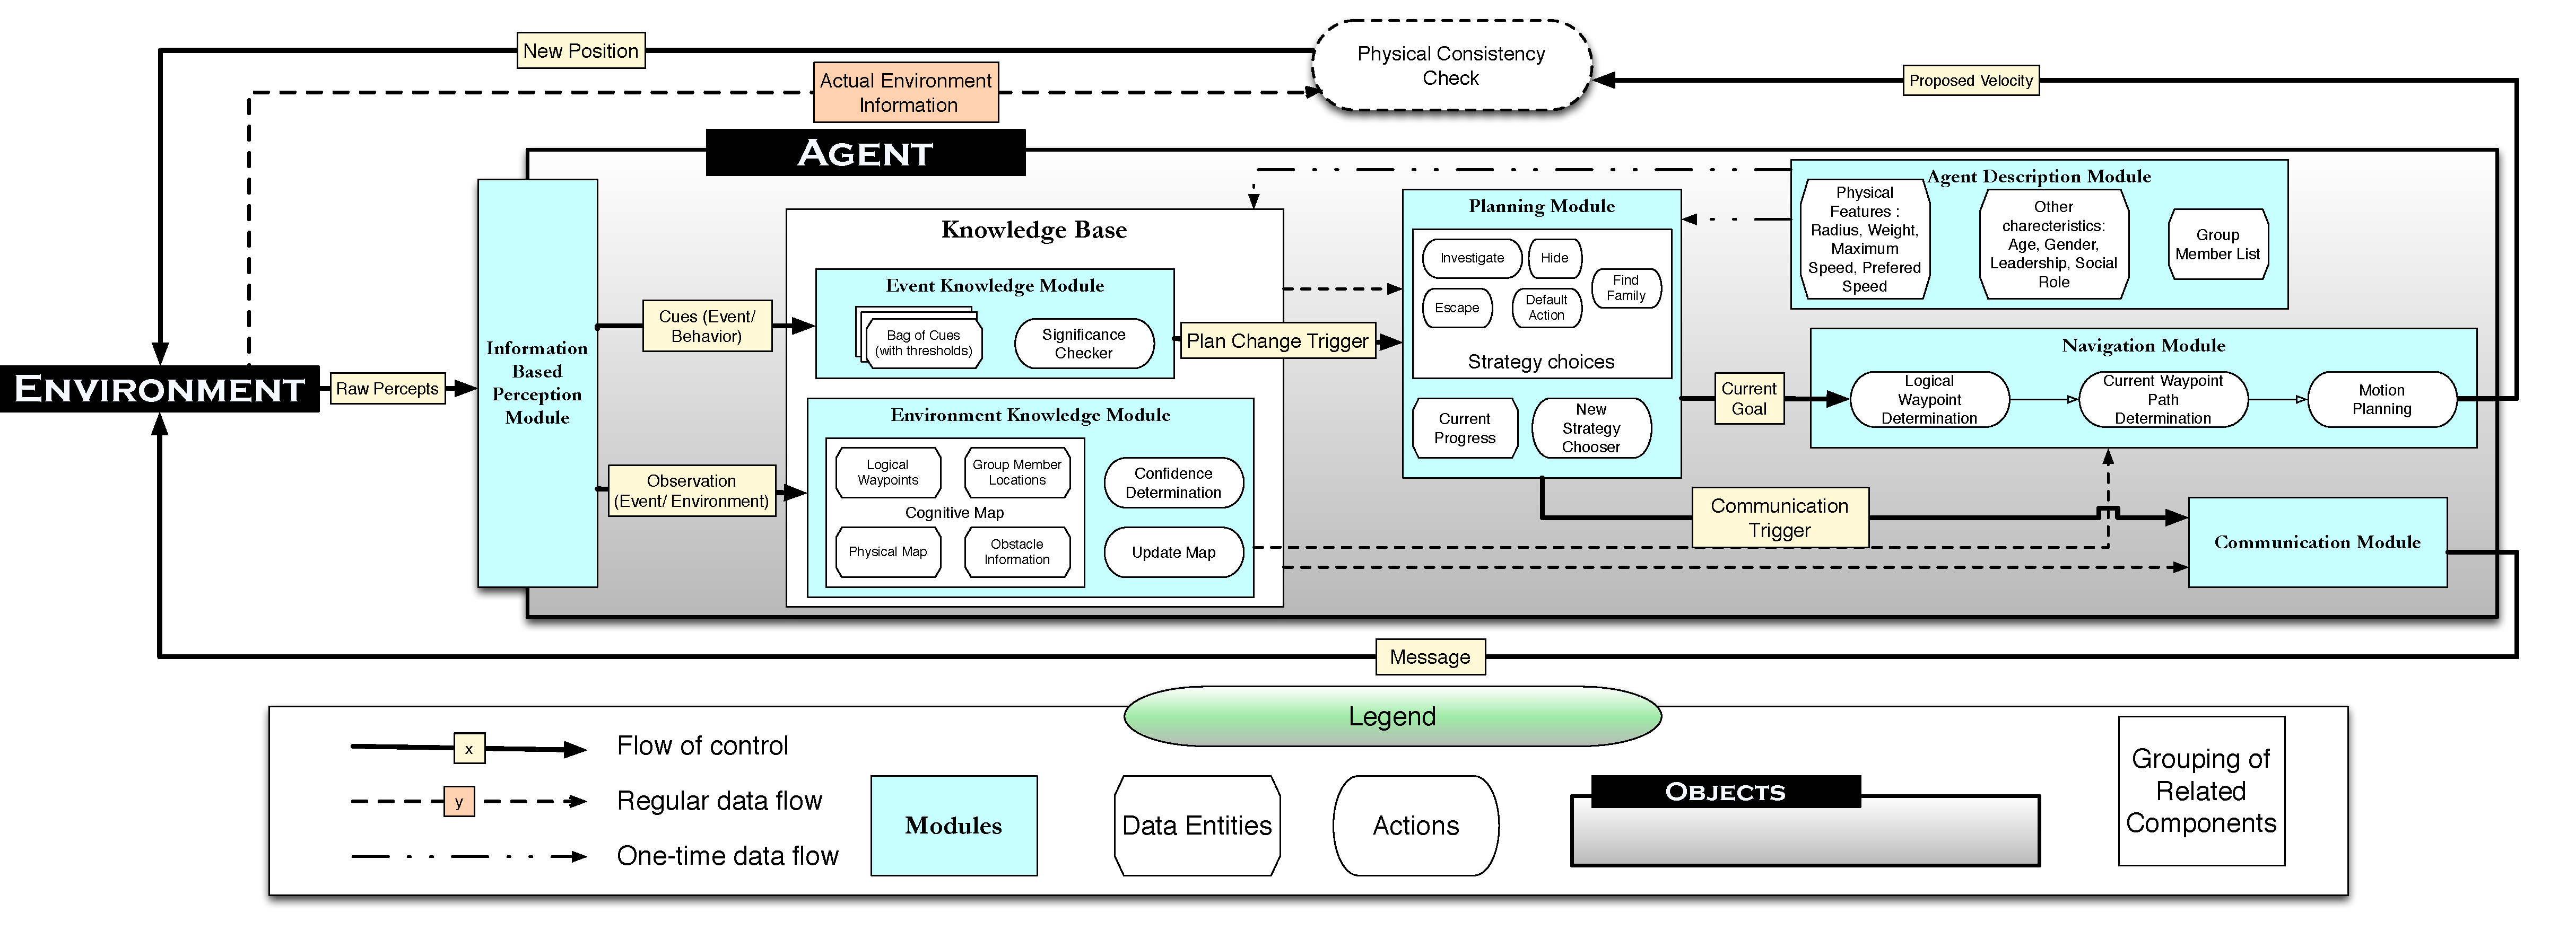
\includegraphics[width=\textwidth]{fig-AgentArchitecture}
\caption[The Agent Architecture]{An illustrated representation of the agent architecture described in Sect.~\ref{IBEVAC:AgentArchitecture}}
\label{fig:AgentArchitecture}
\end{sidewaysfigure}

\subsection{Information Based Perception~(IBP) Module}
\label{IBEVAC:IBPModule}
There are many objects or actions that an agent can sense or observe in the environment. We call these \emph{raw percepts}. There are many different ways according to which these raw percepts can be classified. According to the sources, they can be classified as \emph{observations} from the environment and \emph{messages} from other agents.

Observations themselves can either be observations about the static objects in the environment or the actions of other agents in the environment~(a group of people running away from something). Regardless of the kind of message, in our model, the Information Based Perception~(IBP) module is the only gateway through which the agent receives information from the environment. This module ensures a cap on the amount of information that the agent can process at any given time. Given the kind of information present in the percept, the IBP module passes this on to either the Knowledge Base or the Navigation Module. The working of module is described in detail in Chapter~\ref{chapter:IBP}.

\subsection{Knowledge Base}
\label{IBEVAC:KnowledgeBase}
The Knowledge Base is responsible for storing the beliefs of the agent. It stores all the information that the agent currently has about the environment and the situation. This information or knowledge consists of two things: Event Knowledge and the Environment Knowledge.

\subsubsection{Environment Knowledge Module}
\label{IBEVAC:EnvironmentKnowledgeModule}
The \emph{Environment Knowledge Module} stores the agents personal map. This map is the representation of the layout of the environment that the agent is trying to escape. It is formed as a result of the observations and experiences of the agent in the environment. This module also holds information about the last known locations of the primary group members, so that they can be found in case of an emergency. A confidence value is associated with different areas of the personal map to indicate the amount of confidence the agent has in his own beliefs about the environment. This Environment Knowledge Module also stores information on \emph{landmarks} which indicate areas of the map that the agent believes is accurately represented by itself. This module is discussed in more detail in Sect.~\ref{CFW:EnvironmentKnowledgeModule}.

\subsubsection{Event Knowledge Module}
\label{IBEVAC:EventKnowledgeModule}
The Event Knowledge Module stores the agent's beliefs about the current state of the environment. In a fire evacuation scenario, this module stores information on the current stage in egress that the agent is at. It consists of multiple \emph{buckets} of information each with a specified threshold. Each bucket signifies the belief of the agent that a particular stage in egress has been reached. The value of these thresholds are determined by the Agent Description Module. An overflowing bucket triggers the planner to change its current plan. Each event or behavioral cue that the Event Knowledge Module receives is placed into one of the buckets. Once the amount of information available from the cues in the bucket crosses the threshold a trigger is sent to the planner. This module is discussed in more detail in Sect.~\ref{CFW:EventIdentification}.

\subsection{Agent Description Module~(ADM)}
\label{IBEVAC:AgentDescriptionModule}

This module describes the agent. It explains the properties/~characteristics of the agent. This includes the features of the individual like age, gender, speed, mass and height. It also includes a list of the other members of its predefined primary group. The agent also stores its social role which influences the action it takes in the case of different events. Someone with a social role requiring responsibility will have more high priority tasks relating to helping others. As mentioned earlier, all these factors influence the thresholds in the Event Knowledge Module. Some of these factors are given in Table~\ref{tab:Cues}. This module is discussed mode in Sect.~\ref{CFW:ADM}

\subsection{Planning Module}
\label{IBEVAC:PlanningModule}
The Planning Module creates a plan of action for the agent as a set of tasks. In the current scenario each \emph{task} is just a location that the agent has to go to. This goal is passed to the Navigation Module to determine how exactly to get to that location. The Planning module is shaped by the Agent Description Module, triggered by the Event Knowledge Module and informed by the Environment Knowledge Module. Generally, the planning module has \emph{strategies} for normal action, investigation, finding friends, escaping and taking shelter. Each strategy, while not described completely, does give a set of tasks that the agent is supposed to complete for that strategy and this might vary according to the internals of the ADM. The tasks involved in \emph{investigation} would be to find locations of exits and friends and to verify the existence of fire. The planner, based on the information that it has, will determine the location on the map to move to in order to get the next task done and pass this as the current goal to the Navigation Module. By controlling the state of the agent, the planning module is also indirectly responsible for determining communication. Depending on the type of agent and its state a communication trigger is sent to the communication module to communicate messages with other agents. This module is discussed in more detail in Sect.~\ref{CFW:Planner}.

\subsection{Communication Module}
\label{IBEVAC:CommunicationModule}
 The agents are given an ability to communicate with each other when they are in each other's vicinity. They are thus able to transfer their knowledge of exits and hazards in the environment to others. This mechanism of knowledge transfer is not a straightforward procedure because of the inaccuracies in the personal maps of both the agents and their limited confidence in their own and others' personal maps.

 This module encodes the information passed to it from the Knowledge Base and converts it into messages that can be perceived by other agents' IBP module. It transmits this messages to agents within a communication range provided some conditions are met. This process of communication is explained in more detail in Sect.~\ref{CFW:CommunicationModule}.

\subsection{Navigation Module}
\label{IBEVAC:NavigationModule}

To recap, navigation is defined as the process or activity of accurately ascertaining one's position and planning and following a route. Thus we use the term \emph{Navigation} to refer to the complete process of how a person moves from one point to another. From the definition, Navigation consists of 2 distinct processes: planning a route and following the route. The former is referred to as path planning and the latter is called motion planning.

At the path planning level, the module receives a goal from the Planning Module and it outputs a path that will lead it to this goal. It provides a set of way points to move through to reach this goal. These way points are determined based on the agent's personal map~(from the Environment Knowledge Module) and the obstacles that the agent is currently perceiving~(from the IBP module). In Fig.~\ref{fig:AgentArchitecture}, this module is further broken down into two parts: A higher level path finder that finds abstract logical waypoints towards the goal and a lower level \emph{concrete way point determiner} that translates these logical waypoints to physical locations on the map that the agent can pass through for a collision free path to it's goal.

Motion planning is a term borrowed from robotics which originally means detailing a task into discrete motions. In the context of crowd simulation, we use the term motion planning to refer to the task of finding a collision free velocity to get from the current point to the next waypoint in the planned path. In Fig.~\ref{fig:AgentArchitecture}, the motion planning layer ensures that the agent manages to reach its next way point without colliding with another agent. It takes as input the agent's personal space factor from the ADM and the list of obstacles perceived from the IBP and its knowledge of obstacles from the Environment Knowledge Module and outputs a collision free velocity. A review of existing literature in motion planning is provided in Section~{SectionIBP:MotionPlanning}

At the lowest level a Physical Consistency Check Layer is implemented to provide a sanity check for the model. This layer takes as input the velocity proposed by the collision avoidance layer and makes sure that it does not produce unrealistic behavior by ensuring that people cannot pass through other solid obstacles. This layer does not use the personal map for its calculations, rather it uses the actual map as indicated in Fig.~\ref{fig:AgentArchitecture}. In the figure, this is drawn outside the agent's architecture because the check is done at a global level and does not use any of the agents' individual charecteristics. The dotted border is to indicate that it is still an integral part of the navigation system used by the agents.


The complete process of navigation is discussed in more detail in Sect.~\ref{CFW:NavigationModule}

\section{Summary}
\label{IBEVAC:Summary}

This chapter started with a scenario of what happens to an individual who's involved in a fire evacuation. This was followed by an analysis of the process of evacuation which also proposed how the whole process of evacuation can be explained on the basis of 6 \emph{building blocks}. The next section explained how these 6 building blocks could be translated into an agent architecture. This architecture consisted of \emph{Information Based Perception Module} as a sensor, a \emph{Knowledge Base} consisting of both events and the environment, an \emph{Agent Descriptor Module} which could be used to specify the heterogeneity in the agents, a \emph{Planning Module} for planning and a \emph{Navigation Module} and \emph{Communication Module} as actuators. In the following chapters each of these individual modules will be explained and analyzed in detail. The aim of this report is to develop each of these components to form.